%!TEX root = ../dissertation.tex

\chapter{Modelli per il Bin Packing}\label{chap:four}
In questo capitolo presenteremo prima una rapida introduzione ai modelli matematici per poi analizzare nel dettaglio ciascun modello utilizzato spiegando vincolo per vincolo il loro funzionamento.

\section{Modelli di programmazione matematica}
Quando si parla di problemi di ottimizzazione spesso si fa riferimento alla ricerca operativa e ai modelli matematici, questi modelli producono una soluzione che  massimizza o minimizza una funzione obiettivo su un certo dominio, questa funzione può rappresentare un aspetto di costo o guadagno,  inoltre la soluzione restituita la proprietà di restituire una soluzione ottima. La funzione obiettivo solitamente viene rappresentata come segue:
$$ max\; z = f ( x )\;\; (oppure\; min\; z = f ( x ))$$
s.t.
$$g_i (x) = \begin{cases} \leq b_i \\ = b_i, & i = 1,\dots,m \\ \geq b_i \end{cases}$$
$$x = (x_1,\dots,x_n) \in X \subseteq \mathbb{R}^n$$
In un modello sono presenti:
\begin{itemize}
	\item \textbf{Variabili decisionali}: sono variabili con un dominio prefissat, vengono utilizzate per formulare tutti gli altri elementi del modello, agendo sui valori assunti dalle stesse si troverà la soluzione ottima;
	\item \textbf{Funzione obiettivo}: funzione che deve essere massimizzata o minimizzata in base agli altri elementi su un dominio dato;
	\item \textbf{Vincoli}: serie di vincoli che correlano tra loro le variabili decisionali e permettono di descrivere condizioni fisiche o requisiti particolari richiesti dalla soluzione.
\end{itemize}
\section{Modelli di programmazione lineari}
Particolari tipi di problemi di programmazione matematica sono quelli in cui la funzione obiettivo $f(x)$ e i vincoli $g_i(x)$ sono funzioni lineari, in tal caso si può parlare di modello di \textit{programmazione lineare}, espresso nel seguente modo:
$$ max\; z = \sum_{j=1}^n c_j x_j $$
s.t.
$$\sum_{j=1}^n a_{ij} x_j = \begin{cases} \leq b_i \\ = b_i, & i = 1,\dots,m \\ \geq b_i \end{cases}$$
$$x = (x_1,\dots,x_n) \in X \subseteq \mathbb{R}^n$$
Nonostante i modelli non lineari siano a volte molto più compatti ed intuivi da capire, i modelli lineari mantengono comunque semplicità e sono facilmente risolvibili, sono molti i solver \glo{commerciali} e \glo{open source} disponibili per la loro risoluzione, quello utilizzato durante lo stage è il solver open source di programmazione lineare intera CBC scritto in C++ con interfacciato con Python grazie a Or-Tools. La creazione di un modello lineare parte dall'osservazione di un problema reale, fissando un obiettivo e creando vincoli che descrivano i requisiti estratti dal problema reale astraendo il tutto ad un insieme di vincoli lineari.
Ogni variabile può avere un dominio differente, continua ($x_j \in \mathbb{R}$), intera positiva ($x_j \in \mathbb{Z}^+$) o binaria ($x_j \in \{0,1\}$) a seconda dell'utilizzo che si deve farne.

\section{Modello 2D}
Il modello 2D considera solo larghezza e profondità degli oggetti e non ne permette la rotazione, l'idea di base è quella di considerare solo la \textit{visione aerea} del contenitore che viene così approssimata ad un rettangolo, questo rettangolo ha larghezza (width) prefissita e profondità (depth) infinita, le due dimensioni posso essere considerate come assi di un piano cartesiano aventi origine nel punto di intersezione tra i due assi.\\
\begin{figure}[!h]
	\begin{center} 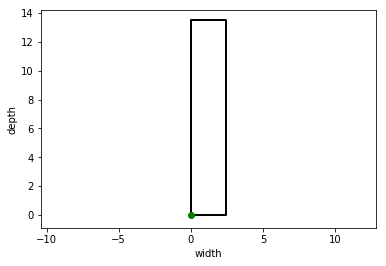
\includegraphics[scale=0.6]{figures/cartesian_wd}
		\caption[Veduta area - piano cartesiano]{Veduta area del container, piano cartesiano con origine nel punto verde.}  
		\label{fig:myInlineFigure}
	\end{center}
\end{figure}

\noindent Per comodità visiva il container non è infinito ma di

\noindent Il modello consiste delle seguenti variabili continue positive:
\begin{itemize}
	\item la variabile intera $x_{i}$ con $i \in I$ individua la coordinata sull'asse x dell'angolo in basso a sinistra dell'oggetto i;
	\item la variabile intera $y_{i}$ con $i \in I$ individua la coordinata sull'asse y dell'angolo in basso a sinistra dell'oggetto i;
\end{itemize}
Il modello consiste delle seguenti variabili binarie:
\begin{itemize}
	\item la variabile binaria $l_{ij}$ con $i,j \in I$ assume il valore 1 se l'oggetto i è situato alla sinistra dell'oggetto j, altrimenti è 0;
	\item la variabile binaria $b_{ij}$ con $i,j \in I$ assume il valore 1 se l'oggetto i è situato al di sotto dell'oggetto j, altrimenti è 0.
\end{itemize}

\begin{equation}
	\begin{aligned}
		& \underset{}{\text{min}} & & D\\
		  & \text{s.t.} &   & l_{ij} + l_{ji} + b_{ij} + b_{ji} \geq 1 & i < j    &   & i,j \in I \\
		  &             &   & y_i - y_j + M_d b_{ij} \leq M_d - d_i    &          &   & i,j \in I \\
		  &             &   & x_i - x_j + M_w l_{ij} \leq M_w - w_i    &          &   & i,j \in I \\
		  &             &   & x_i + w_i \leq W                         &          &   & i \in I   \\
		  &             &   & y_i + d_i \leq D                         &          &   & i \in I   \\
		  &             &   & b_{ij}, l_{ij} \in \{0,1\}               & i \neq j &   & i,j \in I \\
		  &             &   & x_{i}, y_{i} \in \mathbb{R}^{+}          &          &   & i \in I   \\
	\end{aligned}
\end{equation}

\newpage

\section{Modello 2D con rotazione}
Il modello 2D con rotazione introduce in più rispetto al precedente le seguenti variabili binarie:
\begin{itemize}
	\item la variabile binaria $r_{i}$ assume il valore 1 se l'oggetto i è rutotato su se stesso di $90^{\circ}$, ne risulta che $w_{i}$ e $d_{i}$ sono invertiti, altrimenti è 0;
\end{itemize}

\begin{equation*}
	\begin{aligned}
		& \underset{}{\text{min}}
		& & D \\
		  & \text{s.t.} &   & l_{ij} + l_{ji} + b_{ij} + b_{ji} \geq 1                  & i < j    &   & i,j \in I \\
		  &             &   & y_i - y_j + M_d b_{ij} \leq M_d - d_i (1 - r_i) - w_i r_i &          &   & i,j \in I \\
		  &             &   & x_i - x_j + M_w l_{ij} \leq M_w - w_i (1 - r_i) - d_i r_i &          &   & i,j \in I \\
		  &             &   & x_i + w_i (1 - r_i) + d_i r_i \leq W                      &          &   & i \in I   \\
		  &             &   & y_i + d_i (1 - r_i) + w_i r_i \leq D                      &          &   & i \in I   \\
		  &             &   & b_{ij}, l_{ij}, r_i \in \{0,1\}                           & i \neq j &   & i,j \in I \\
		  &             &   & x_{i}, y_{i} \in Z^{+}                                    &          &   & i \in I   \\
	\end{aligned}
\end{equation*}

\newpage

\section{Modello 2D con rotazione e sequenza scarico}
Con questo modello ci proponiamo di disporre nel miglior modo possibile gli oggetti sul pianale del camion tenendo conto anche della sequenza di scarico, un oggetto può essere scaricato lateralmente da destra o da sinistra, oppure dal fondo del camion. \\
Nel momento in cui l'oggetto verrà scaricato questo dovrà avere almeno una di queste vie libere affinché possa essere scarico. \\
L'indice $v \in \Omega = \{1,2,3\}$ rispettivamente $v = 1$ si indica la direzione sinistra, $v = 2$ si indica la direzione destra ed infine $v = 3$ si indica la direzione di fronte a sè. \\
Il modello 2D con rotazione e sequenza scarico introduce in più rispetto al precedente le seguenti variabili binarie:
\begin{itemize}
	\item la variabile binaria $\alpha_{ij}$ assume il valore 1 se l'oggetto i ha alla sua sinistra l'oggetto j e questo gli impedisca di essere sfilato lateralmente, altrimenti è 0;
	\item la variabile binaria $\beta_{ij}$ assume il valore 1 se l'oggetto i ha alla sua destra l'oggetto j e questo gli impedisca di essere sfilato lateralmente, altrimenti è 0;
	\item la variabile binaria $\gamma_{ij}$ assume il valore 1 se l'oggetto i ha davanti a se l'oggetto j e questo gli impedisca di essere sfilato centralmente, altrimenti è 0;
	\item la variabile binaria $s_{vi}$ assume il valore 1 se l'oggetto i ha nella direzione v almeno un oggetto che gli impedisca di essere sfilato nella rispettiva direzione, altrimenti è 0;
\end{itemize}
Inoltre si fa riferimento anche ad alcuni pamarametri:
\begin{itemize}
	\item la parametro binario $o_{ij}$ assume il valore 1 se l'oggetto i appartiene ad un ordine che deve essere scaricato prima dell'ordine a cui appartiene l'oggetto j, altrimenti è 0;
\end{itemize}

\begin{equation*}
	\begin{aligned}
		& \underset{}{\text{min}}
		& & D \\
		& \text{s.t.} & &  l_{ij} + l_{ji} + b_{ij} + b_{ji} \geq 1 & i < j && i,j \in I \\
		& & & y_i - y_j + M_d b_{ij} \leq M_d - d_i (1 - r_i) - w_i r_i & & & i,j \in I \\
		& & & x_i - x_j + M_w l_{ij} \leq M_w - w_i (1 - r_i) - d_i r_i & & & i,j \in I \\
		& & & x_i + w_i (1 - r_i) + d_i r_i \leq W & & & i,j \in I \\
		& & & y_i + d_i (1 - r_i) + w_i r_i \leq D & & & i,j \in I \\
		  &   &   & \alpha_{ij} \leq l_{ij}                             &   &   & i,j \in I &   & \hypertarget{(1.1)}{(1.1)} \\
		  &   &   & \alpha_{ij} \leq 1 - (b_{ij} + b_{ji})              &   &   & i,j \in I &   & \hypertarget{(1.2)}{(1.2)} \\
		  &   &   & \alpha_{ij} \geq l_{ij} - M_\alpha(b_{ij} + b_{ji}) &   &   & i,j \in I &   & \hypertarget{(1.3)}{(1.3)} \\
		  &   &   & \beta_{ij} \leq l_{ji}                              &   &   & i,j \in I &   & \hypertarget{(2.1)}{(2.1)} \\
		  &   &   & \beta_{ij} \leq 1 - (b_{ij} + b_{ji})               &   &   & i,j \in I &   & \hypertarget{(2.1)}{(2.1)} \\
		  &   &   & \beta_{ij} \geq l_{ji} - M_\beta(b_{ij} + b_{ji})   &   &   & i,j \in I &   & \hypertarget{(2.2)}{(2.2)} \\
		  &   &   & \gamma_{ij} \leq b_{ij}                             &   &   & i,j \in I &   & \hypertarget{(3.1)}{(3.1)} \\
		  &   &   & \gamma_{ij} \leq 1 - (l_{ij} + l_{ji})              &   &   & i,j \in I &   & \hypertarget{(3.2)}{(3.2)} \\
		  &   &   & \gamma_{ij} \geq b_{ij} - M_\gamma(l_{ij} + l_{ji}) &   &   & i,j \in I &   & \hypertarget{(3.3)}{(3.3)} \\
		& & & \alpha_{ij}o_{ij} \leq s_{1i}  & & & i,j \in I \\
		& & & \beta_{ij}o_{ij} \leq s_{2i}  & & & i,j \in I \\
		& & & \gamma_{ij}o_{ij} \leq s_{3i}  & & & i,j \in I \\
		  &   &   & \sum_{v \in \Omega} s_{vi} \leq 2                   &   &   & i \in I   &   & (4)                        \\
		& & & b_{ij}, l_{ij}, r_i \in \{0,1\} & i \neq j & & i,j \in I \\
		& & & x_{i}, y_{i} \in Z^{+} & & & i \in I \\
		  &   &   & s_{vi} \in \{0,1\}                                  &   &   & i \in I   &   & v\in \Omega                \\
	\end{aligned}
\end{equation*}

Le disequazione \hyperlink{(1.1)}{(1.1)},\hyperlink{(1.2)}{(1.2)},\hyperlink{(1.3)}{(1.3)}  

\section{Modello 3D con rotazione e sovrapposizione}
Con questo modello, evoluzione del modello 2D con rotazione, ci si propone di introdurre la sovrapposizione degli oggetti, considerando però che alcuni oggetti potranno avere come condizione quella di non poter avere altri oggetti sopra di sè. Un problema non indifferente inerente questo modello viene individuato nella stabilità degli oggetti, soluzioni che riportino oggetti sopraelevati, le cui aree di base non poggino completamente sugli oggetti sottostanti sono da ritenersi non valide. Per risolvere questo problema si è deciso di optare per una semplificazione, se un oggetto i si trova sopra ad un oggetto j, allora l'area di base dell'oggetto i dovrà essere interamente appoggiata alla faccia superiore dell'oggetto j.
Il modello 3D con rotazione e sovrapposizione introduce in più rispetto al precedente le seguenti variabili intere:
\begin{itemize}
	\item la variabile intera $z_{i}$ individua la coordinata sull'asse z dell'angolo in basso a sinistra dell'oggetto i;
\end{itemize}
Introduce in più rispetto al precedente anche le seguenti variabili binarie:
\begin{itemize}
	\item la variabile binaria $t_{ij}$ assume il valore 1 se l'oggetto i ha sopra di sè l'oggetto j, altrimenti è 0;
	\item la variabile binaria $f_{ij}$ assume il valore 1 se l'oggetto i ha sopra di sè l'oggetto j e la faccia superiore dell'oggetto i è a contatto con la faccia inferiore dell'oggetto j, altrimenti è 0;
\end{itemize}
Inoltre la variabile binaria $k_{ij}$ viene utilizzata per imporre che un oggetto possa trovarsi alla sinistra o dietro ad un altro oggetto ma non al di sotto di un altro e videversa, imponendo ciò che segue:
\begin{itemize}
	\item \textbf{$k_{ij} = 1 \Rightarrow$} $t_{ij} + t_{ji} = 0 \land l_{ij} + l_{ji} + b_{ij} + b_{ji} = 1$
	\item \textbf{$k_{ij} = 0 \Rightarrow$} $t_{ij} + t_{ji} = 1 \land l_{ij} + l_{ji} + b_{ij} + b_{ji}= 0$
\end{itemize}

\begin{equation*}
	\begin{aligned}
		& \underset{}{\text{min}}
		& & D \\
		& \text{s.t.} & & k_{ij} \leq l_{ij} + l_{ji} + b_{ij} + b_{ji} & i < j && i,j \in I \\
		& & & 2 k_{ij} \geq l_{ij} + l_{ji} + b_{ij} + b_{ji} & i < j && i,j \in I \\
		& & & 1 - k_{ij} = t_{ij} + t_{ji} & i < j && i,j \in I \\
		& & & y_i - y_j + M_d b_{ij} \leq M_d - d_i (1 - r_i) - w_i r_i & & & i,j \in I \\
		& & & x_i - x_j + M_w l_{ij} \leq M_w - w_i (1 - r_i) - d_i r_i & & & i,j \in I \\
		& & & h_i - h_j + M_h t_{ij} \leq M_h - h_i & & & i,j \in I \\
		& & & h_i - h_j + M_h f_{ij} \geq - M_h - h_i & & & i,j \in I \\
		& & & x_i - x_j \leq M_w (1-f_{ij}) & & & i,j \in I \\
		& & & y_i - y_j \leq M_d (1-f_{ij}) & & & i,j \in I \\
		& & & z_i + h_i \leq H & & & i \in I \\
		& & & f_{ij} \leq t_{ij} & & & i \in I \\
		  &   &   & M_h \sum_{i \in I} f_{ij} \geq z_j &   &   & i \in I &   & (4) \\
		& & & x_i + w_i (1 - r_i) + d_i r_i \leq W & & & i,j \in I \\
		& & & y_i + d_i (1 - r_i) + w_i r_i \leq D & & & i,j \in I \\
		%& & & x_i - x_j + w_i(1-r_i) + d_i r_i - w_j(1-r_j) - d_j*r_j \geq - Mw(1 - f_{ij}) & & & i,j \in I\\
		%& & & y_i - y_j + d_i(1-r_i) + w_i r_i - d_j(1-r_j) - w_j*r_j \geq - Md(1 - f_{ij}) & & & i,j \in I\\
		& & & b_{ij}, l_{ij}, t_{ij}, f_{ij}, k_{ij} \in \{0,1\} & i \neq j & & i,j \in I \\
		& & & x_{i}, y_{i}, z_{i}, r_{i} \in Z^{+} & & & i \in I \\
	\end{aligned}
\end{equation*}

\section{Big M}
Le Big M, dato che hanno dimostrato di essere un elemento di forte influenza rispetto il tempo di ricerca della soluzione ottima, sono state definite cercando di restringere il loro dominio nel seguente modo:
\begin{itemize}
	\item M: dato gli n oggetti, M è la somma della massima dimensione tra $w_i$ e $d_i$ dell'oggetto i-esimo;
	\item $M_w$: viene definito come la larghezza del camion W sommato ad M;
	\item $M_d$: viene definito come la profondità del camion D sommato ad M.
\end{itemize}
